\chapter{Realizing a Two-Qubit Processor} \label{chapter:design}

This chapter discusses the design and fabrication processes of the two-qubit processor used in this thesis work. We start by introducing the general constraints faced when designing our two-qubit processor, followed by a component-wise discussion of its individual parts and the associated parameters we need to choose for them.

\section{Introduction \& Motivation}

\begin{figure}[ht!]
  \centering
	\includegraphics[width=1.\textwidth]{"./material/figures/2-qubit-processor/processor_schematic_parameters"}
	\caption[Circuit schematic of the two-qubit processor]{The circuit schematic of the two-qubit processor used in this work, together with all parameters that have to be chosen. Shown are the two Transmon qubits in green, the drive and readout circuit in blue, the fast flux lines in red and the coupling capacitance in magenta.}
	\label{fig:2_qubit_chip_circuit_diagram}
\end{figure}

As discussed in the introduction, the most simple imaginable quantum processor consists of two qubits that can be manipulated and read out individually, and between which one can realize a universal two-qubit gate. We implement such a two-qubit processor using two Transmon qubits that are coupled by a fixed capacitor and that can be read out out individually by a pair of cavity Josephson bifurcation amplifiers (CJBAs). Figure \ref{fig:2_qubit_chip_circuit_diagram} shows the circuit diagram of our processor with all relevant design parameters. Shown are the two qubits in green, the drive and readout circuit in red, the coupling capacitance between them in magenta, and in red fast flux lines required to tune the qubit frequencies (as we show below).

\subsection{Processor Operation}

\begin{figure}[ht!]
	\centering
	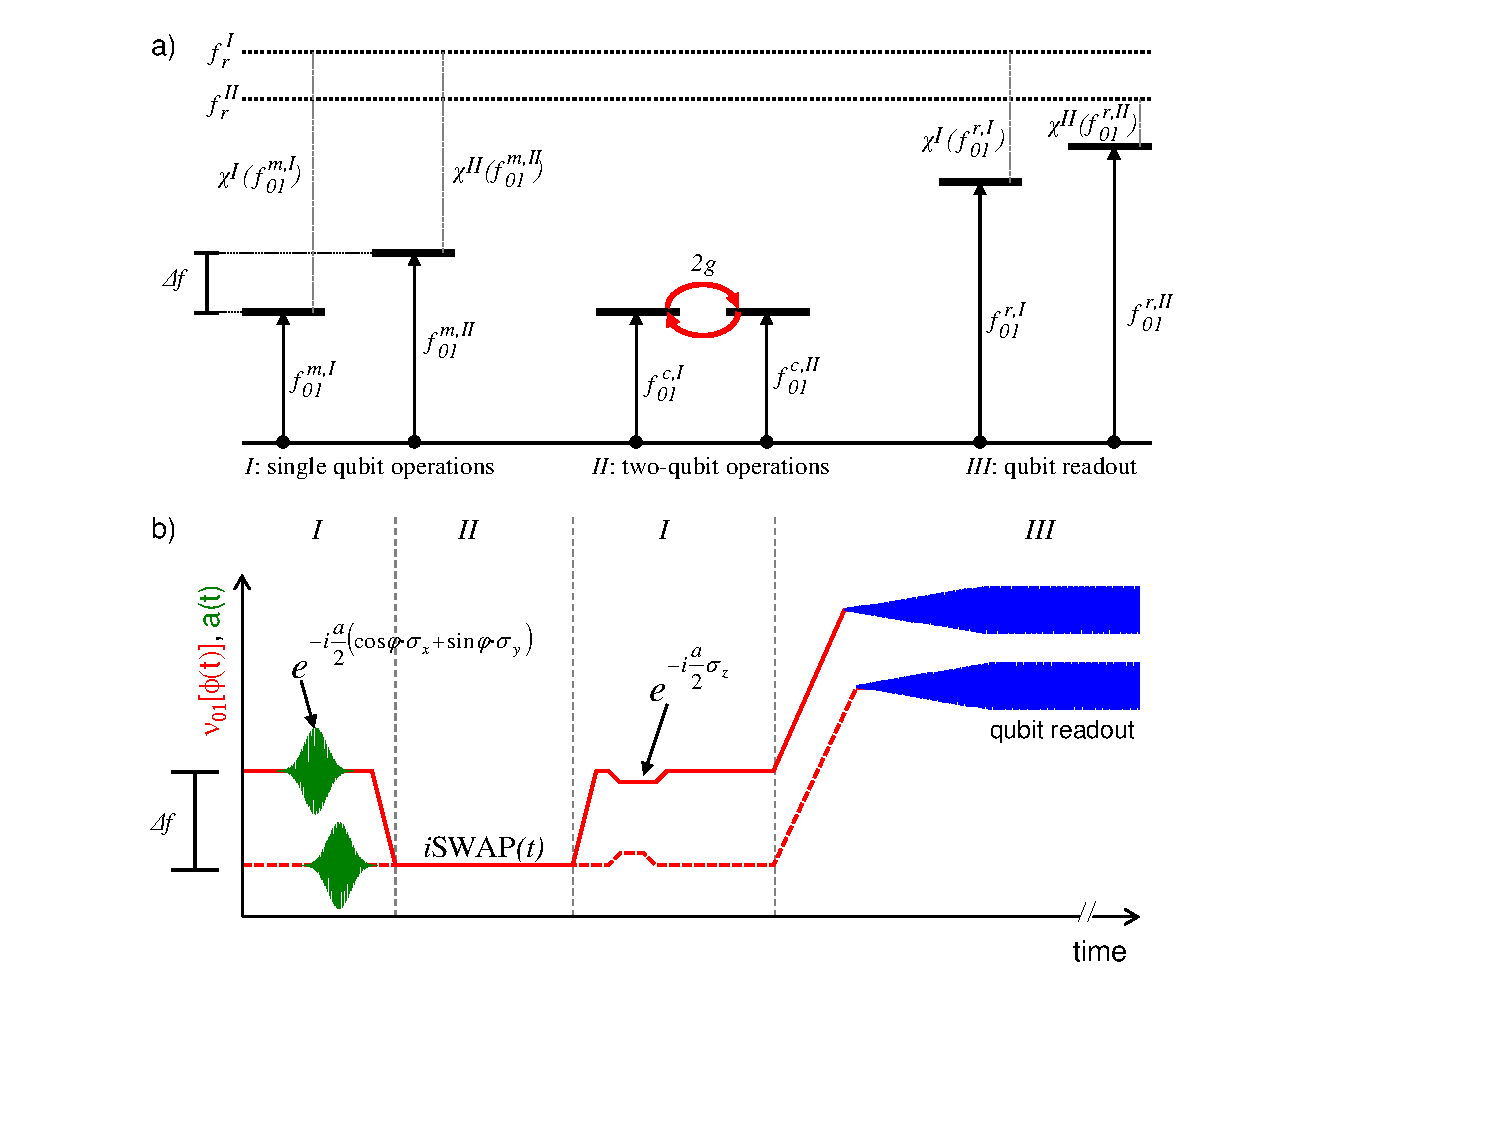
\includegraphics[width=\textwidth]{./material/figures/2-qubit-processor/processor_working_principle}
	\caption[...]{Operation principle of the two-qubit processor. a) The qubit frequencies for different operations. I: Single-qubit manipulation and parking. II: Two-qubit coupling. III: Qubit readout. For each operation, different qubit frequencies are chosen, resulting in different qubit-qubit coupling and qubit-readout couplings $\chi_r^{I,II}(f_{01}^{I,II}$. b) Typical gate sequence illustrating the different operations. The sequence consists of two single-qubit XY-gates, a two-qubit $i\mathrm{SWAP}(t)$ gate, two single-qubit Z-gates and ends with the qubit readout.}
	\label{fig:processor_operation}
\end{figure}

We want to perform three basic operations with the quantum processor:

\begin{itemize}
\item \textbf{Single-qubit gates}: Manipulating a single qubit by rotating its Bloch vector around the $X$, $Y$ or $Z$ axis of the Bloch sphere.
\item \textbf{Two-qubit gate}: Performing a (universal) two-qubit gate, in this work in particular the $\sqrt{i\mathrm{SWAP}}$ and $i\mathrm{SWAP}$ gates.
\item \textbf{Qubit readout}: Performing single-shot readout of the state of each qubit, possibly simultaneously for both of them.
\end{itemize}

The parameter requirements for each of these operations are usually conflicting: For single-qubit manipulation, no interaction between the qubits must be present, hence the qubit frequencies need to be strongly detuned. However, to implement the two-qubit gates, strong resonant interaction between the qubits is required, hence the two qubit frequencies should be resonant. Furthermore, during qubit manipulation the relaxation of the qubit state through the readout resonator should be negligible, hence the frequency detuning $\Delta$ between each qubit and its readout resonator should be large, as shown by eq. (\ref{eq:purcell_rate}). On the other hand, to obtain a high state fidelity during the readout of the qubit state, the interaction between the qubit and its readout resonator should be large, which requires a small frequency detuning $\Delta$ between the two.

\smallskip

We solve these conflicting requirements by dynamically changing the qubit frequencies during the operation of the processor using fast on-chip flux lines. Fig. \ref{fig:processor_operation} illustrates this basic operating principle of the two-qubit processor: For each of the three basic operations (single-qubit manipulation, two-qubit gate and readout), we choose a different set of qubit frequencies $f_{01}^{I,II}$. For the single-qubit gates, the two frequencies $f_{01}^{m,I}$ and $f_{01}^{m,II}$ are detuned by $\Delta f_m = f_{01}^{m,II}-f_{01}^{m,I}$. This tuning is chosen such that only negligible qubit-qubit interaction is present when performing single-qubit manipulations or no operation. Furthermore, at this working point the detuning between each qubit and its readout resonator is such that the qubit lifetime is not limited by relaxation through the gate circuit. To realize a two qubit gate, the two qubits get tuned in resonance such that $f_{01}^{c,I} = f_{01}^{c,II}$. At this point, the qubits experience a swapping interaction as given by eq. (\ref{eq:cqed_qubit_interaction_hamiltonian}) with an effective swapping frequency $2g$. For the readout, we change the qubit frequencies to $f_{01}^{r,I}$, $f_{01}^{r,II}$, reducing the qubit-resonator detuning such that the corresponding dispersive shift $\chi^I(f_{01}^{r,I})$ and $\chi^{II}(f_{01}^{r,II})$ of the resonator during readout assures an optimal readout fidelity. The displacement of the qubit frequency between the different working points has to be performed on a time scale faster than all relevant qubit manipulation and coupling frequencies but not as a fast as to induce transitions of the qubit state.

\smallskip

We discuss now the parameters of each component of the processor in greater detail, explaining each time the relevant design goals and possible conflicts and presenting the parameter choice or compromise we arrive at.

\section{Qubit Design}

The main design goals for the qubits are large coherence times, good frequency tunability and the possibility of fast single-qubit driving. Good frequency tunability is important since we need to move the qubits to different frequency working points for single-qubit and two-qubit manipulation as well as qubit readout. The maximum qubit drive frequency should be large compared to the decoherences times of the qubit, so that we are able to perform a large number of gate operations on the qubit before its coherence is destroyed, which is crucial when running quantum algorithms.

\subsection{Qubit Frequency \& Junction Asymmetry}

The choice of the maximum qubit frequency is influenced by several requirements:

\begin{itemize}
\item The density of thermal photons at the qubit frequency should be sufficiently low at the operating temperature of the circuit (typically 20-100 mK) such that the thermal excitation of the qubit into higher energy levels is negligible.
\item Robust equipment for signal generation and measurement in the frequency range of the qubit should be available. This includes microwave sources needed to generate the charge drive pulses as well as room-temperate and cryogenic microwave components such as mixers, splitters, circulators and amplifiers.
\item The design of microwave circuits is all the more easy, the lower the required frequency range.
\end{itemize}

In addition, the choice of the qubit frequency also influences the choice of the readout resonator frequency. For our qubits, we choose a minimum transition frequency of $\omega_{01}^{1,2}/2\pi= 4 \;\mathrm{GHz}$, which ideally yields a negligible excited state occupation probability of $p(\ket{1})=1/[1+\exp{(\hbar \omega / k_B T)}]=2.1\%$ at $T=50\;\mathrm{mK}$. In addition, in the frequency range $2-18\;\mathrm{GHz}$, commercial microwave equipment and components are available for both room-temperature as well as cryogenic applications. A qubit frequency tunability bandwidth of 3 GHz being sufficient for the operation of the processor, we choose a maximum qubit frequency $\omega_{01}^{max}/2\pi = 7\;\mathrm{GHz}$.

\smallskip

As described in chapter \ref{chapter:theory}, we use a split Josephson junction geometry as shown in fig. \ref{fig:cpb_circuit}b to make the Josephson energy of the qubit tunable by an external flux $\Phi_{ext}$. The modulation depth of $E_J(\Phi_{ext})$ is given by eq. (\ref{eq:josephson_energy_modulation}): The higher the junction asymmetry $d$, the smaller the modulation depth of the Josephson energy $\simeq 1-d$. In general, it can be advantageous to operate the qubit at a working point where $\partial E_J(\Phi)/\partial \Phi=0$ since at that point the qubit will be insensitive to flux noise at first order. Hence we chose an asymmetry $d\approx 0.35$ so that the minimum qubit frequency coincides with our lower boundary frequency of $4\;\mathrm{GHz}$.

\subsection{Single-Qubit Gates} \label{section:qubit_driving}

We distinguish between single-qubit rotations around the $X$ and $Y$ axes and around the $Z$ axis of the Bloch sphere. The latter are implemented by changing the qubit frequency using a fast on-chip flux line, whereas the former are implemented by driving the qubit with an oscillatory electrical drive signal at its resonance frequency. For the $X/Y$ gates, it is necessary to capacitively couple the qubit to an external charge driving circuit. 

\paragraph{Charge Driving} 

The maximum drive frequency of the qubit is limited by its anharmonicity: Since the Transmon qubit is only weakly anharmonic, when driving the qubit at a frequency comparable to the qubit anharmonicity, transitions to higher Transmon levels will be induced, therefore producing a leakage of the qubit state out of the computational basis and hence unitary drive errors. This effect can be partially alleviated by increasing the anharmonicity of the qubit. However, by increasing the anharmonicity, one also increases the sensitivity of the qubit to charge noise. Hence it is necessary to find a compromise for the value of the qubit anharmonicity which allows sufficiently fast qubit driving but which does not incur too much dephasing.

\smallskip

To estimate the drive error arising due to the finite anharmonicity of a Transmon, we model its driving using a simple three-level Hamiltonian in the rotating-frame, as used e.g. in \cite{motzoi_simple_2009}:
%
\begin{equation}
\hat{H} = \alpha\left(
						 \begin{array}{ccc}
						0 & \epsilon^*(t)/\alpha & 0 \\
						\epsilon(t)/\alpha & \delta/\alpha & \sqrt{2}\epsilon^*(t)/\alpha \\
						0 & \sqrt{2}\epsilon(t)/\alpha & 2\delta/\alpha + 1
						\end{array}
					\right) \label{eq:qubit_three_level_driving_hamiltonian}
\end{equation}
%

Here, $\epsilon(t) = \epsilon_x(t)+i\epsilon_y(t)$ is the complex drive IQ amplitude in the rotating qubit frame, $\delta$ is the detuning of the microwave drive from the Transmon $\omega_{01}$ transition frequency and $\alpha$ is the Transmon anharmonicity. Due to the presence of the third energy level, the effective $\ket{0}\to\ket{1}$ transition frequency will get shifted with respect to the bare frequency $\omega_{01}$ when driving the qubit. For $\delta = \alpha = 0$, the characteristic polynomial of $\hat{H}$ is given as $E(E^2-3|\epsilon|^2/4) = 0$ with the two eigenvalues $E=\pm |\epsilon|\sqrt{3}/2$. Thus, for weak anharmonicities this frequency shift is given approximately as $\Delta_{ac}=\sqrt{3}|\epsilon|/2$. To estimate the leakage to the Transmon level $\ket{2}$ when driving the system, we calculate the eigenvalues and eigenvectors of the Hamiltonian (\ref{eq:qubit_three_level_driving_hamiltonian}). We then decompose an initial state $\ket{0}$ in the basis of eigenstates of $\hat{H}$ and calculate its evolution operator $U_d(t,\delta,\epsilon_0)$ under a constant drive amplitude $\epsilon_0$. By numerically maximizing the occupation probability of the state $\ket{1}$ as a function of the evolution time $t$ and the drive detuning $\delta$ we obtain the ideal gate time, gate error and frequency shift for a $\pi$-pulse at a given drive frequency/anharmonicity ratio. In fig. \ref{fig:three_level_driving_errors} we show these quantities as a function of $\epsilon/\alpha$. As can be seen, the gate error due to leakage into the level $\ket{2}$ increases with the drive frequency. For very large drive frequencies, the gate fidelity saturates at a value of $F\approx 0.86$ (the numerically obtained maximum $\pi$-pulse fidelity for ultra-strong driving of the three-level system is $F_{max}\approx 0.895$). We can make use of fig. \ref{fig:three_level_driving_errors} to estimate the minimum required qubit anharmonicity given the desired gate fidelity and gate time. If we demand a maximum Rabi frequency $\epsilon/2=\Omega_{Rabi}^{max}=2\pi\cdot 100\;\mathrm{MHz}$, which corresponds to a gate time for a single-qubit $\pi$-pulse of $T_\pi=5\;\mathrm{ns}$ small compared to the targeted relaxation and dephasing times of the qubit of $T_1,T_\phi\simeq 1\;\mathrm{\mu s}$, and a maximum $\pi$-gate error of $1-F_\pi = 0.04$, we need an absolute anharmonicity $\alpha > 250\;\mathrm{MHz}$.

\smallskip

It is possible to correct leakage errors using optimized DRAG drive pulses \cite{lucero_reduced_2010,chow_optimized_2010}, thereby eliminating leakage to the third qubit level. In this work, we did not use such techniques but we will  include possible errors arising due to this leakage to higher Transmon levels in our error models when discussing experimental data.

\begin{figure}[htp!]
	\centering
	\includegraphics[width=\textwidth]{"./material/mathematica/three_level_driving_errors"}
	\caption[Single-qubit $\pi$-pulse gate time, gate fidelity and AC stark detuning as a function of drive strength]{The single-qubit $\pi$-pulse gate time, gate fidelity and AC Stark detuning, plotted as a function of the reduced drive strength $\epsilon/\alpha$ applied to the three-level Transmon. As the drive strength increases, the gate time decreases as $\alpha/\epsilon$ whereas the gate fidelity decreases non-monotonously.}
	\label{fig:three_level_driving_errors}
\end{figure}

\smallskip 

Furthermore, charge driving of the qubit is done through the readout resonator on the chip, as shown in fig. \ref{fig:2_qubit_chip_circuit_diagram}. The Rabi frequency of the qubit in eq. (\ref{eq:drive_hamiltonian}) is given as $\Omega_{Rabi}= 2 \beta e V_d \bra{0}\hat{n}\ket{1}$, where the drive voltage $V_d$ seen at the qubit gate capacitance depends on the input voltage $V_{in}$ at the input capacitance of the resonator as given by eq. (\ref{eq:qubit_drive_voltage}). Since the resonator acts as a band-pass filter for the input drive signal, the more the drive frequency $\omega_d$ is detuned from the resonator frequency $\omega_r$, the smaller the gate voltage seen by the qubit is. A Rabi frequency of $\Omega_{Rabi}^{max}/2\pi=100\;\mathrm{MHz}$ at $\omega_{01}/2\pi=4\;\mathrm{GHz}$ corresponds to $V_{in}=0.4\;\mathrm{mV}$ for the resonator parameters that we will choose below, $\omega_r/2\pi = 6.7\;\mathrm{GHz}$, $g_{01}/2\pi=50\;\mathrm{MHz}$ and $Q=800$. With 70 dB attenuation inside the cryostat this corresponds to an input power of $P\approx 15\;\mathrm{dBm}$ at room temperature, which is compatible with our microwave setup.

\paragraph{Flux Driving}

To rapidly change the flux in the qubit loop, we couple each qubit inductively to a fast flux line. The flux induced in the qubit loop by this line is given as $\Phi_{ext}=M I_{fl}$, where $I_{fl}$ is the current in the line and $M$ is the mutual inductance between the flux line and the qubit loop, which can be estimated as $M=\mu_0 l \ln{\left[(d_f+w)/d\right]}/2\pi$, where $l$ is the length of the qubit loop parallel to the flux line, $d_f$ the distance of the loop to the line and $w$ the width of the qubit loop perpendicular to the flux line. In order to avoid sample heating through the flux line, we demand a maximum current for inducing one flux quantum $\Phi_0$ in the loop not in excess of $I_{\Phi_0}^{max}=10\;\mathrm{mA}$, corresponding to an electrical input power of $P^{max}_{in}=50\;\mathrm{mW}$ on a $50 \; \Omega$ transmission line with 20 dB attenuation and $P^{max}_{out}=500\;\mathrm{\mu W}$ on the output transmission line, which can be easily dissipated on the 1 K stage of the cryostat. This yields a minimal value of the mutual inductance $M\ge 0.23\;\mathrm{pH}$, which can easily be achieved with a qubit loop of $l=w=4\;\mathrm{\mu m}$ at a distance $d_f=12\;\mathrm{\mu m}$ to the flux line. The coupling of the qubit to the flux line also induces decoherence that we will take into account later when confirming our choice of $M$.

\smallskip

In general, when passing a low-frequency or DC current through the flux line, superconducting shielding currents will build up in the ground plane around the line. Therefore, we usually remove the ground plane between the center pin of the flux line and the qubit loop, since otherwise the induced shielding currents will modify the effective flux seen by the qubit and lead to unwanted distortions in the shape of the applied flux signal. However, removing this ground plane also leads to stronger capacitive coupling of the qubit to the flux line, thereby increasing qubit relaxation, which we also have to take into account.

\subsection{Qubit-Qubit Coupling}

\begin{SCfigure}[1.0][hbt!]
	\centering
	\begin{tabular}{l}
	a) \\ 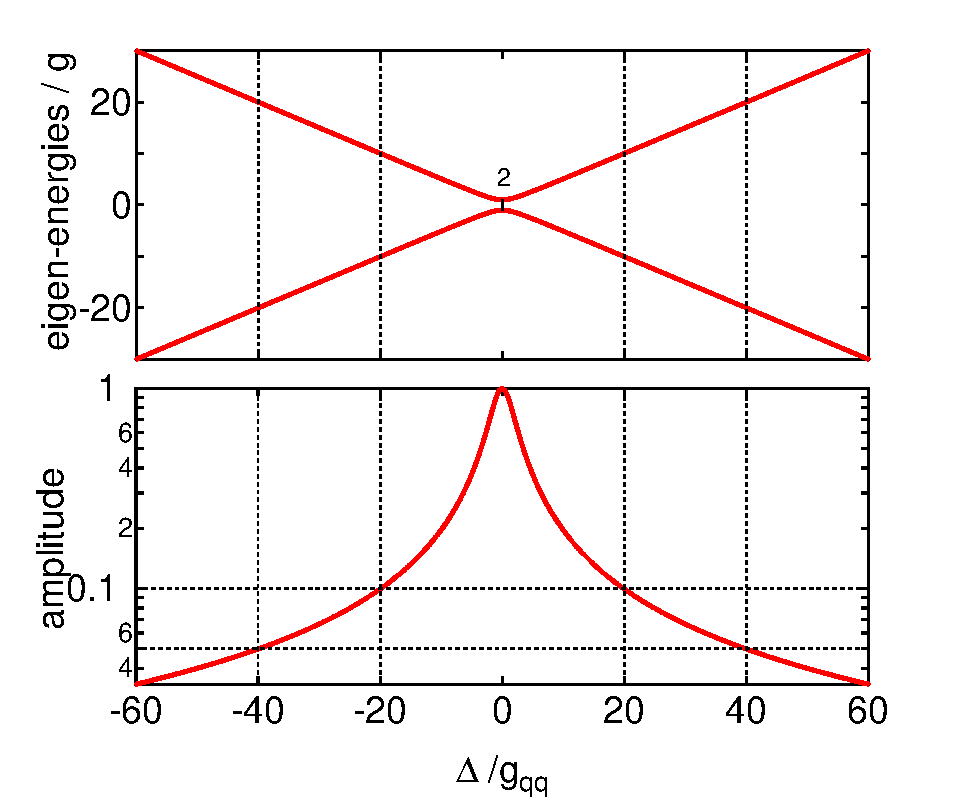
\includegraphics[width=0.49\textwidth]{./material/mathematica/qubit_qubit_coupling} \\
	b) \\ 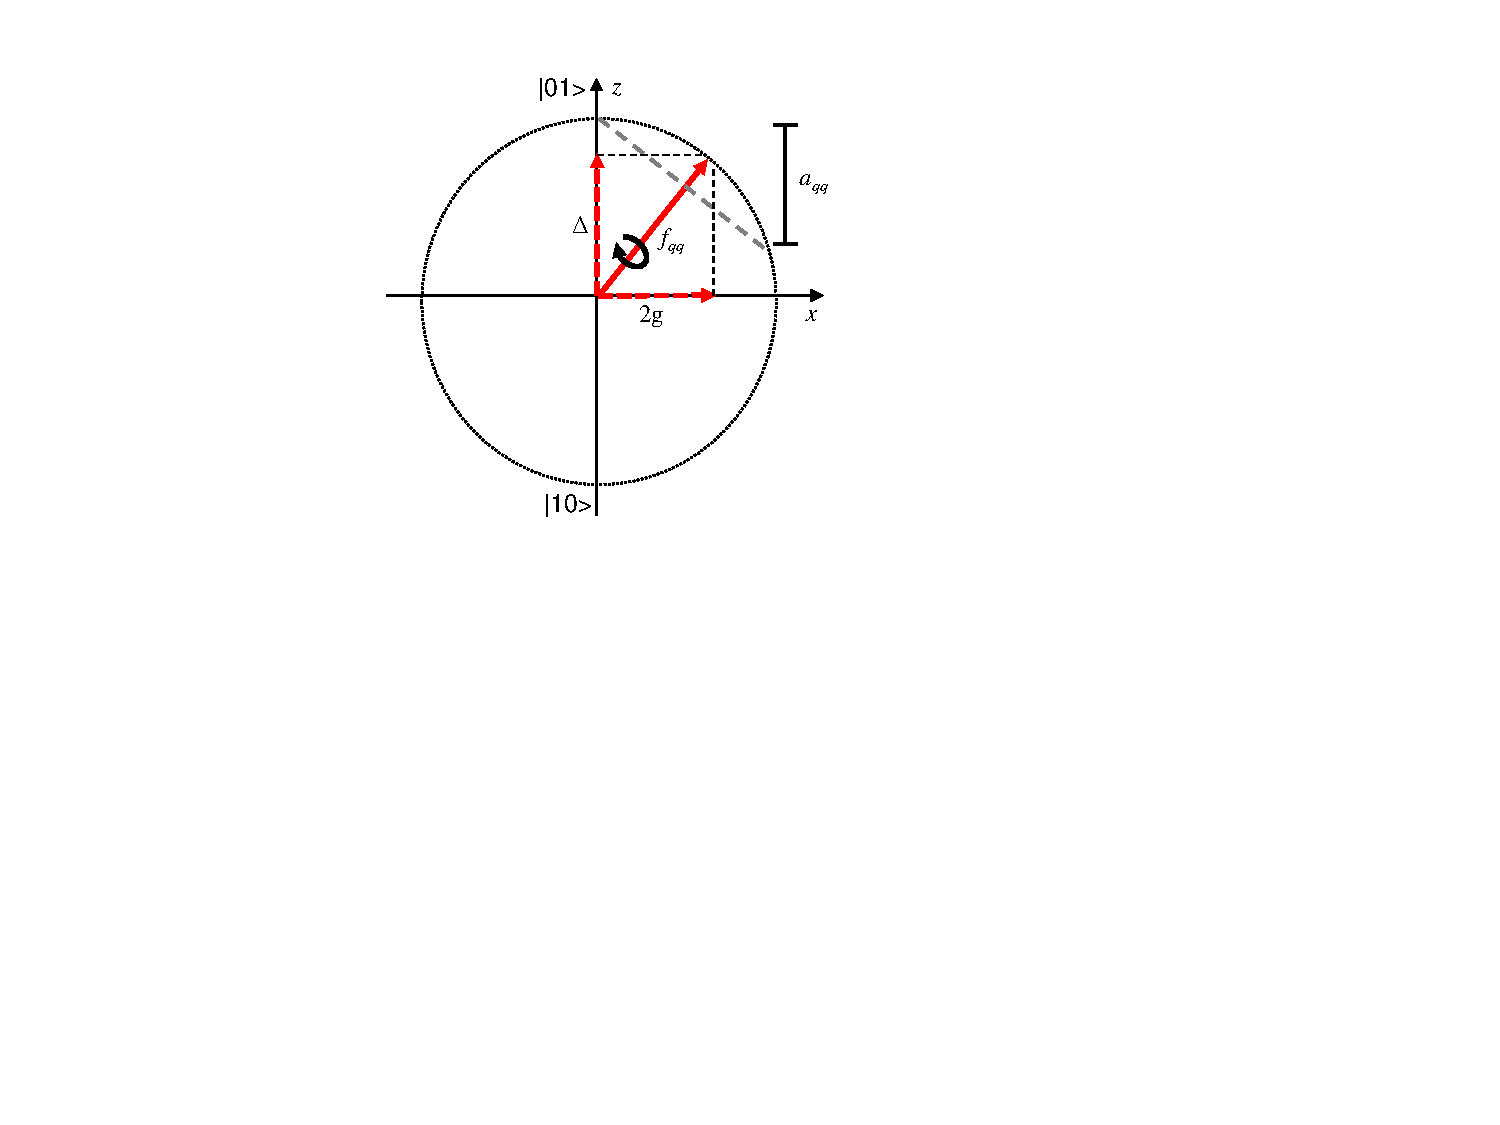
\includegraphics[width=0.49\textwidth]{./material/figures/introduction/bloch_sphere_coupling_illustration}
	\end{tabular}
	\caption[]{a) The two-qubit eigen-energies $E_\pm$ and swapping amplitude $a_{qq}$ as given by eqs. (\ref{eq:qubit_coupling_amplitude_and_frequency}). For $\Delta \gg g$, the amplitude of the swap decreases $\propto 1/\Delta$ and the frequency increases $\propto \Delta$. To effectively switch of the swapping interaction to $a_{qq}=0.1$, a detuning of $\Delta = 20 g$ is required. b) Illustration of the swapping amplitude and frequency on the $\ket{01}$,$\ket{10}$ Bloch sphere: The rotation axis depends on the ratio $\Delta/g$, for $\Delta=0$ it coincides with the $x$ axis whereas for $\Delta \gg g$ it asymptotically approaches the z axis. At the same time, the frequency of rotation around this axis increases $\propto \Delta$. }
	\label{fig:qubit_coupling_amplitude_and_frequency}
\end{SCfigure}

We use a direct capacitive coupling between our qubits to create an interaction between them suitable to implement a two-qubit gate. The full interaction Hamiltonian is given by eq. (\ref{eq:swap_with_detuning}), and the coupling strength $g_{qq}$ between the two qubits can be calculated with eq. (\ref{eq:cqed_capacitive_coupling}). This coupling strength must be chosen such that the interaction between the qubits is sufficiently fast to realize two-qubit gate operations with adequate fidelity, but not too strong in order to still allow to sufficiently suppress the coupling by detuning the qubit frequencies, as needed. By diagonalizing the Hamiltonian (\ref{eq:cqed_qubit_interaction_hamiltonian}) we find for the eigen-energies $E_{qq}^\pm$, the swapping frequency $f_{qq}$ and the swap amplitude $a_{qq}$ of the two coupled qubits as a function of the qubit-qubit detuning $\Delta/2\pi=f_{01}^I-f_{01}^{II}$ the values
%
\begin{eqnarray}
E_{qq}^\pm & = & \pm\frac{1}{2}\sqrt{4g_{qq}^2+\Delta^2}, \notag \\
f_{qq}     & = & \sqrt{4g_{qq}^2+\Delta^2}, \notag \\
a_{qq}     & = & \frac{2g_{qq}}{\sqrt{4g_{qq}^2+\Delta^2}}. \label{eq:qubit_coupling_amplitude_and_frequency}
\end{eqnarray}
%
Figure \ref{fig:qubit_coupling_amplitude_and_frequency} shows the the eigen energies and qubit-qubit swapping amplitude as a function of the normalized qubit-qubit detuning $\Delta/g$. As can be seen, for $\Delta \gg g$ the swap amplitude decreases $\propto 1/\Delta$ whereas the swap frequency increases $\propto \Delta$. For our processor, we demand that the residual swapping amplitude $a\le 0.1$ when the qubits are ``parked'' for single-qubit gates and readout, hence it is necessary to detune the qubits by $\Delta \approx 20 g$. At this detuning, the swapping frequency is given as $f_{qq}(20 g)\approx 20 g$. For our processor, we choose $2g/2\pi = 10\;\mathrm{MHz}$, corresponding to a qubit-qubit detuning of $200\;\mathrm{MHz}$ at $a_{qq}=0.1$ and an associated swapping frequency $f_{qq}=100\;\mathrm{MHz}=(10\;\mathrm{ns})^{-1}$. The required frequency displacement is easily achievable with the on-chip fast flux lines. On resonance, the swap frequency of $10\;\mathrm{MHz}$ allows us to realize an $\sqrt{i\mathrm{SWAP}}$ gate in $25\;\mathrm{ns}$ and an $i\mathrm{SWAP}$ gate in $50\;\mathrm{ns}$, which is sufficiently fast compared to the estimated relaxation and dephasing times of the qubits. The residual swapping between the qubits at their parking position is usually small enough to be irrelevant for most experiments performed in this work. However, when executing long gate sequences, as required for certain algorithms, the induced error may be too large, hence a larger detuning should be chosen for these cases.

\smallskip

To estimate the error due to finite rise times for the flux pulse before the $i\mathrm{SWAP}$ gate, we numerically solve the Schrödinger equation of the 2-qubit system in the $\ket{01},\ket{10}$ basis, which is given as
%
\begin{equation}
i\hbar\left(\begin{array}{c} \dot{\psi}_{01} \\ \dot{\psi}_{10} \end{array}\right) = \left( \begin{array}{cc} -\frac{\Delta(t)}{2} & g \\ g & \frac{\Delta(t)}{2}  \end{array} \right)\cdot \left(\begin{array}{c} \psi_{01} \\ \psi_{10} \end{array}\right) \label{eq:swap_evolution}
\end{equation}
%

\begin{figure}[ht!]
\def\imagetop#1{\vtop{\null\hbox{#1}}}

	\centering
	\begin{tabular}{ll}
	a) & b) \\
	\imagetop{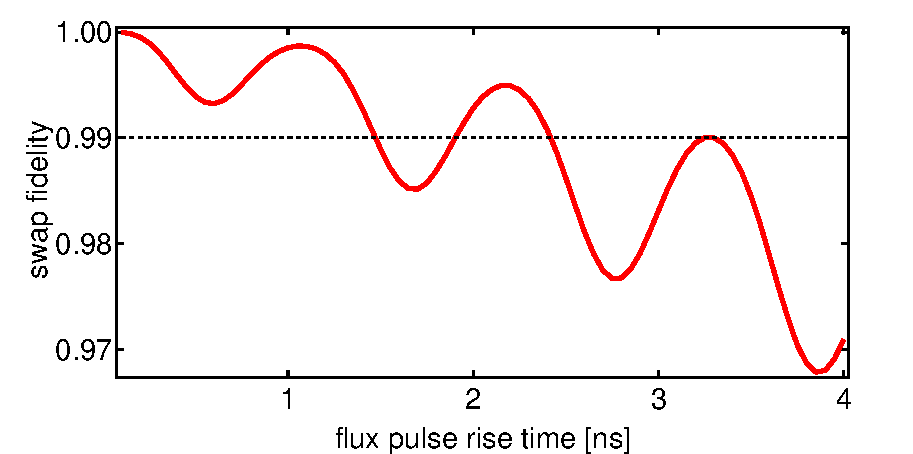
\includegraphics[width=0.6\textwidth]{./material/mathematica/qubit_qubit_swap_error}} &
	\imagetop{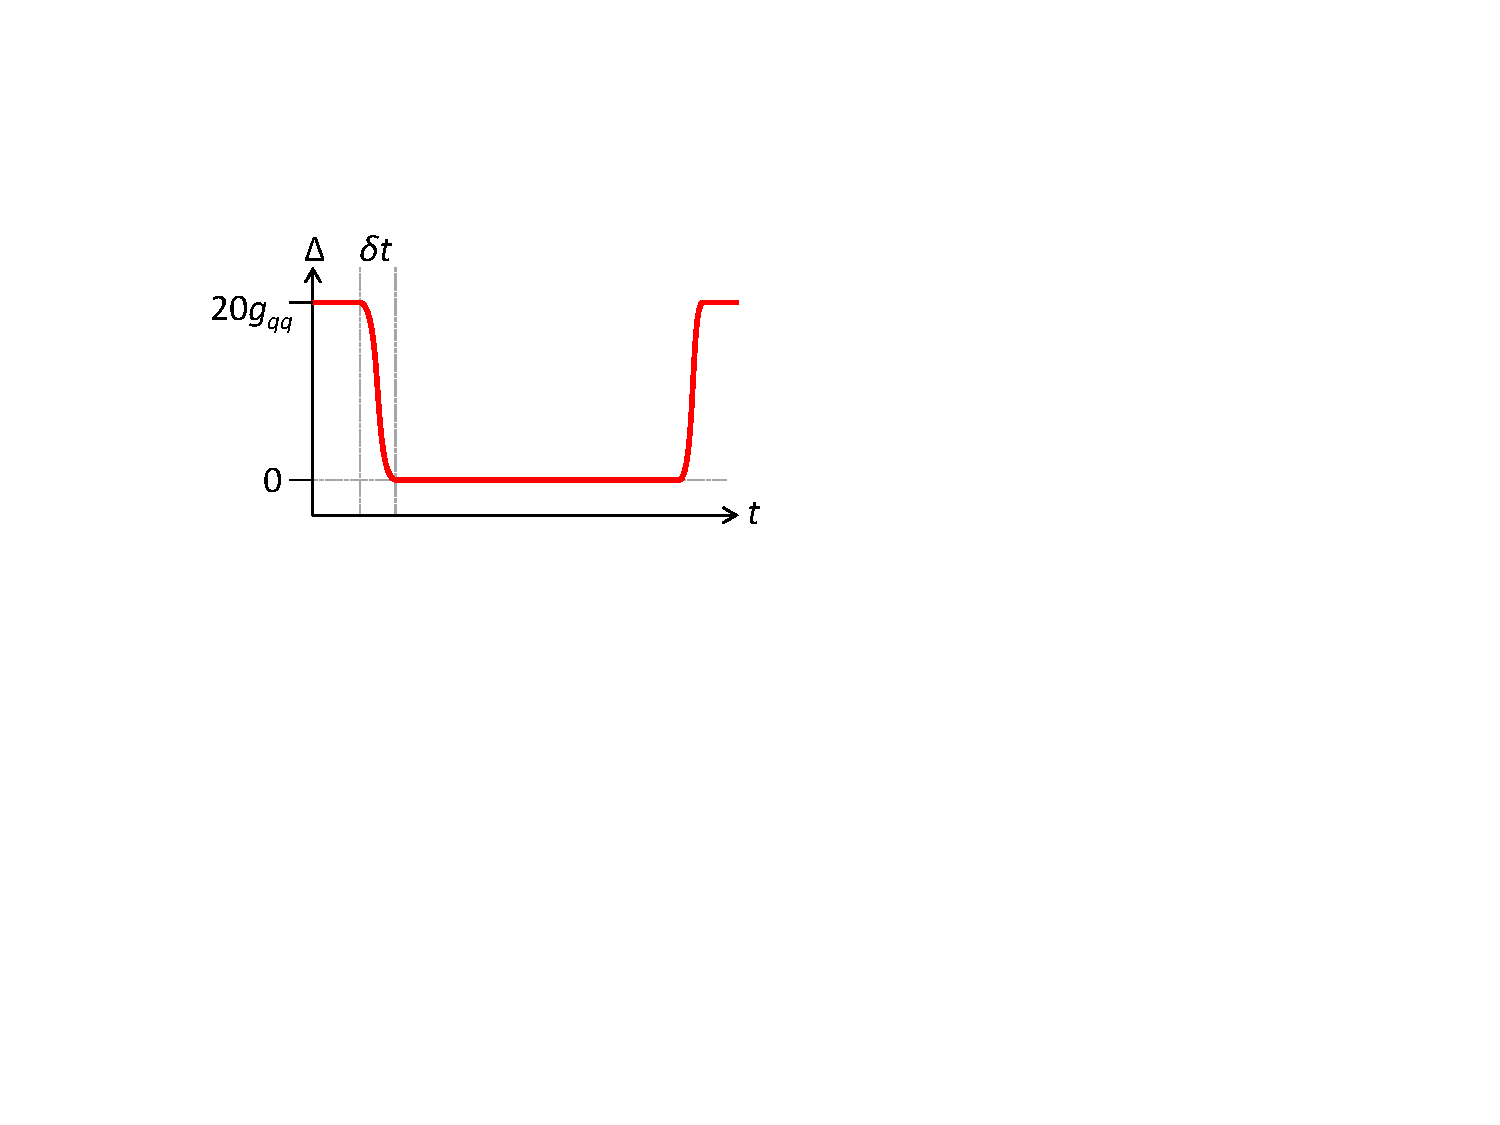
\includegraphics[width=0.4\textwidth]{./material/figures/2-qubit-processor/flux_pulse_rise_time}}
	\end{tabular}
	\caption[]{a) Numerically obtained maximum fidelity of a two-qubit $i\mathrm{SWAP}$ gate realized by changing the detuning $\Delta$ in eq. (\ref{eq:swap_evolution}) from $\Delta = 20g$ to $\Delta=0$ using a Gaussian pulse of width $\delta t$. b) Simulated pulse shape used to obtain the curve shown.}
	\label{fig:qubit_qubit_coupling_swap_error}
\end{figure}

To estimate the error, we go from a detuning $\Delta = 20 g$ at $t=0$ to a detuning $\Delta=0$ using a Gaussian waveform with a rise time $\delta t$. We then numerically determine the maximum SWAP amplitude between the qubits and plot the resulting value against $\delta t$. The result of this simulation is shown in fig. \ref{fig:qubit_qubit_coupling_swap_error}. As can be seen, the fidelity of the gate decreases in a non-monotonous way as a function of the flux pulse rise time. In order to obtain $F>0.99$, a flux pulse rise time of $\delta t \le 1.5\;\mathrm{ns}$ is required.

\subsection{Relaxation and Dephasing}

In this section we discuss the relaxation and dephasing channels of the Transmon qubit which are most relevant to our experiment. We analyze the relaxation and dephasing rates as a function of the Transmon parameters and optimize these parameters to achieve maximum qubit coherence times.

\begin{SCfigure}[1.0][ht!]
	\centering
	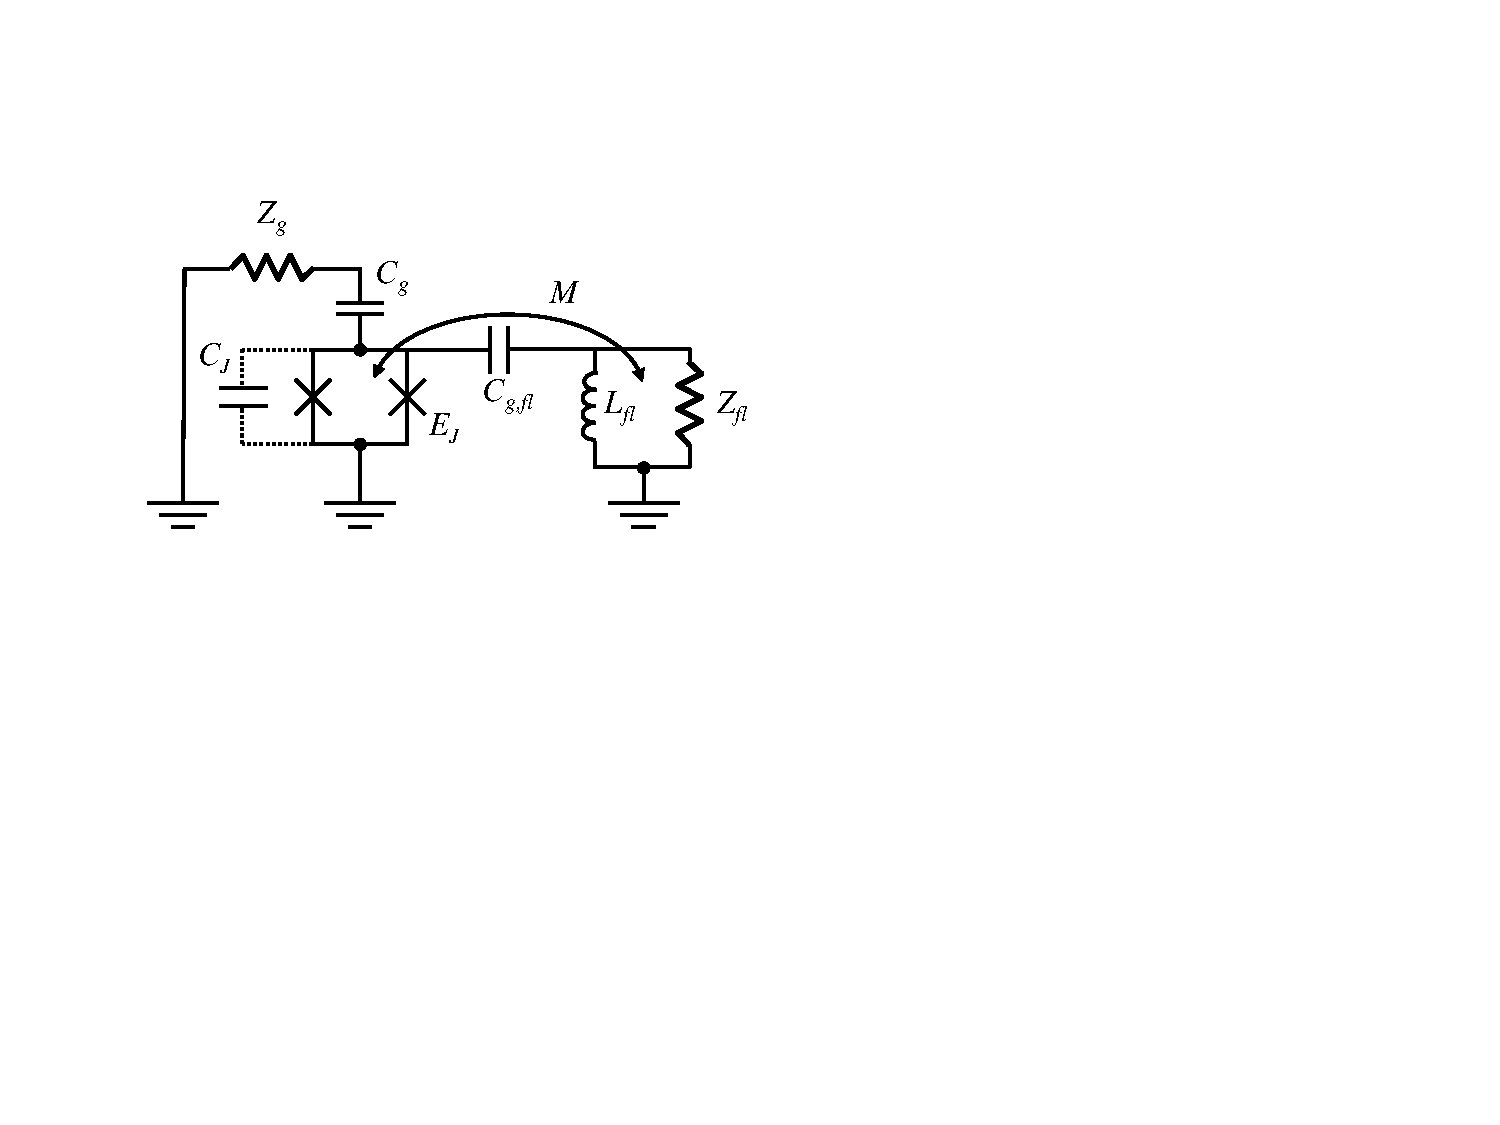
\includegraphics[width=0.6\textwidth]{./material/figures/introduction/cooper_pair_box_decoherence}
	\caption[]{A schematic model showing the coupling of the qubit to its environment, modeled by impedances $Z_g$ and $Z_{fl}$, through capacitive and inductive couplings $C_g$ and $M$.}
	\label{fig:cooper_pair_box_decoherence}
\end{SCfigure}

\subsubsection{Qubit Relaxation}

Relaxation of the qubit can occur either through the charge channel or the flux channel. The qubit has a capacitive coupling to both the flux line and the readout resonator, hence charge relaxation through both of them is possible. On the other hand, the only relevant relaxation channel through the flux channel is through the inductive coupling to the external flux line.

\paragraph{Relaxation through the Gate Charge Channel}

Since the CPB is coupled to an external impedance (in this case the readout resonator that is coupled to a lossy input transmission line) through a gate capacitance $C_g$, as shown in fig. \ref{fig:cooper_pair_box_decoherence}, relaxation into modes of the input impedance seen by the qubit can occur. The relaxation time of the Transmon qubits used in previous experiments was found to be limited to $T_1^{int}=1-4\;\mathrm{\mu s}$ independent of the circuit \citep{simmonds_decoherence_2004,martinis_decoherence_2005}. Consequently, we require the relaxation time associated to charge relaxation through the gate circuit to be significantly longer than this intrinsic relaxation time, i.e. $\Gamma_1^{Purcell}\ll 1\;\mathrm{MHz}$. This requirement influences the choice of the coupling of the qubit to the readout resonator $g_{01}$, the quality factor and associated loss rate $\kappa$ of this resonator and the qubit-resonator detuning $\Delta$ for the different processor operations. The relaxation rate due to the coupling of the qubit to the input resonator is given by eq. (\ref{eq:purcell_rate}). For the qubit parameters chosen above, a resonator quality factor $Q=800$ and a resonator-qubit coupling of $g_{01}/2\pi=50\;\mathrm{MHz}$ chosen below, the relaxation rate is $\Gamma_1^{Purcell}\approx 0.25\;\mathrm{MHz}$ at $\Delta/2\pi = 2\;\mathrm{GHz}$ (for qubit manipulation) and $\Gamma_1^{Purcell}\approx 1\;\mathrm{MHz}$ at $\Delta/2\pi = 1\;\mathrm{GHz}$ (for qubit readout). This rate is comparable or larger than the typical intrinsic relaxation rate of the qubit and thus compatible with our design goals.

\smallskip

In addition to the capacitive coupling to the input impedance $Z_g$, the qubit is also coupled to its flux line by $C_{g,fl}$, which can lead to relaxation through the charge channel of the flux line \citep{johnson_controlling_2010}. Assuming that the flux line is terminated by a 50 $\Omega$ load and that $C_{g,fl}\le 10\;\mathrm{fF}$. yields a relaxation rate $\Gamma_1^{\mathrm{fl},n_g}\le 260 \;\mathrm{kHz}$ for the qubit parameters discussed above, which is lower than the maximum demanded relaxation rate and thus compatible with our design requirements.
 
\paragraph{Relaxation through the Flux Channel} \label{section:relaxation_through_charge}

On the two-qubit chip, each Transmon is equipped with a fast magnetic flux line that is used to perform flux biasing and fast frequency displacements. The flux lines are coupled to the qubits through a mutual inductance $M$, as shown in fig. \ref{fig:cooper_pair_box_decoherence}. The sensitivity of the qubit to relaxation through the flux channel via the mutual inductance $M$ is given by eq. (\ref{eq:flux_relaxation_sensitivity}). For the mutual inductance discussed above, $M \approx 0.23\;\mathrm{pH}$, a characteristic impedance of the flux line of $Z_{fl}=50\;\Omega$, a qubit frequency $\omega_{01}/2\pi= 7 \;\mathrm{GHz}$ and anharmonicity $\alpha=-250\;\mathrm{MHz}$ and an asymmetry $d=0.35$, we obtain a maximum relaxation rate of $\Gamma_1^{fl}=0.28\;\mathrm{MHz}$, which is small compared to all other relevant relaxation rates. This rate represents an upper bound for an unfiltered flux line, in our experiment the low-pass filtering of the line will further decrease this rate by decreasing $\mathrm{Re}(1/Z_{fl}(\omega_{01}))$ at the qubit frequency $\omega_{01}$. We confirm therefore our choice of the mutual inductance $M=0.25\;\mathrm{pH}$ for the flux coupling of the qubit. 

\subsubsection{Qubit Dephasing}

Dephasing of the qubit can occur due to coupling to external charge or flux noise. Here we will calculate the associated rates for both cases for our designed qubit parameters.

\paragraph{Dephasing through the Flux Channel}

For the qubit parameters discussed in the last paragraph, using eq. (\ref{eq:flux_dephasing_rate}) we obtain a maximum dephasing rate $\Gamma_\phi^{\delta \phi_{ext}}= 0.3\;\mathrm{MHz}$ in the relevant frequency interval $\omega_{01}/2\pi = 4-7 \; \mathrm{GHz}$. This rate is thus smaller than the relaxation-limited dephasing rate of the qubit at all relevant working frequencies of our processor. Our choice of qubit parameters is thus compatible with the demanded dephasing time.

\paragraph{Dephasing through the Charge Channel}

We can use eq. (\ref{eq:charge_dephasing_rate}) to calculate the charge-induced dephasing rate of our Transmon qubit. This rate depends exponentially on the ratio $E_J/E_C$. The highest dephasing rate occurs thus at the smallest qubit frequency that we operate our qubit at, in our case $\omega_{01}/2\pi=4\;\mathrm{GHz}$. The chosen maximum tolerable dephasing rate of $\left(\Gamma_{\phi}^{\delta N_g}\right)^{-1} \approx 1\;\mathrm{\mu s}$ at $\omega_{01}/2\pi=4\;\mathrm{GHz}$ is obtained for a qubit anharmonicity of $\alpha\approx-500\;\mathrm{MHz}$, which is thus the upper bound for the anharmonicity. However, for this work we choose $\alpha=-250\;\mathrm{MHz}$, since it allows already for sufficiently fast driving of the qubit, as discussed in section \ref{section:qubit_driving}. For this parameter choice, we obtain a negligible maximum dephasing rate $\left(\Gamma_{\phi}^{\delta N_g}\right)^{-1} \approx 1\;\mathrm{ms}$ at $\omega_{01}/2\pi=4\;\mathrm{GHz}$. 

\smallskip

As mentioned in section \ref{section:decoherence_in_cqed}, the coupling of the qubit to the readout resonator can induce dephasing trough the AC-Stark shift of the qubit induced by photon-number fluctuations in the resonator. The resulting relaxation rate is given by eq. (\ref{eq:thermal_photon_number_dephasing_rate}). For the qubit parameters discussed above and a qubit-resonator coupling $g_{01}/2\pi=50\;\mathrm{MHz}$, the dephasing rate is $\Gamma_\phi^{\bar{n}}= 0.95\cdot{\bar{n}} \;\mathrm{MHz}$ at the minimum chosen qubit-resonator detuning $\Delta = 1 \;\mathrm{GHz}$. The average number of photons in a resonator with $\omega_{r}/2\pi = 6.7\;\mathrm{GHz}$ at $T=100\;\mathrm{mK}$ is given as $\bar{n} = [\exp{(\hbar\omega_r/k_B T)-1}]^{-1} \approx 0.05$, yielding an effective dephasing rate $\Gamma_\phi^{\bar{n}}\approx 38\;\mathrm{kHz}$, which is small compared to the flux-induced dephasing rate at all working points of the qubit.

\section{Readout Design}

As explained in section \ref{section:jba_operation_principle} of chapter \ref{chapter:theory}, the readout fidelity is influenced by three sources of error: Finite overlap between the switching probability distributions for different qubit states, relaxation of the qubit during the measurement phase of the readout and retrapping of the resonator state during the latching phase of the readout. In order to minimize these errors, the following constraints should be met for the readout resonator:

\begin{enumerate}
\item The state-dependent dispersive shift of the resonator frequency should be large enough such that the switching probability distributions of the resonator corresponding to the qubit states $\ket{0}$ and $\ket{1}$ do not overlap.
\item The measurement phase of the readout should be completed in a time $T_{meas}$ which is short compared to the relaxation time of the qubit, i.e. $T_{meas}\ll T_1$.
\item There should be no retrapping of the resonator state during the latching period of the readout.
\end{enumerate}

In order to maximize the dispersive shift, we can either increase the coupling $g_{01}$ between the resonator and the qubit or reduce the frequency detuning $\Delta$ between them. However, increasing $g_{01}$ or decreasing $\Delta$ will also increase the relaxation rate of the qubit through the Purcell effect, thereby reducing the readout fidelity. There is thus an optimum choice for $g_{01}$ and $\Delta$ \citep{mallet_single-shot_2009}. To counteract the qubit relaxation through the cavity, we can simply increase the quality factor of the resonator. However, usually the maximum relaxation time of the Transmon qubit used in this work is limited to $T_1\approx 1-4\;\mathrm{\mu s}$ due to intrinsic relaxation processes. Therefore, increasing the quality factor of the resonator does not necessarily increase the readout fidelity because a higher quality factor also increases the time required to excite the readout resonator by the drive pulse and hence the measurement time of the qubit state. Therefore, if the qubit relaxation time is intrinsically limited, a longer measurement time at a constant relaxation rate implies a higher probability for the qubit to relax during the measurement, hence actually reducing the readout fidelity. We therefore need to find a compromise for the values of $g_{01}$, $\chi$ and $\Delta$ that will maximize the readout fidelity under the given constraints.

\begin{SCfigure}[1.0][ht!]
	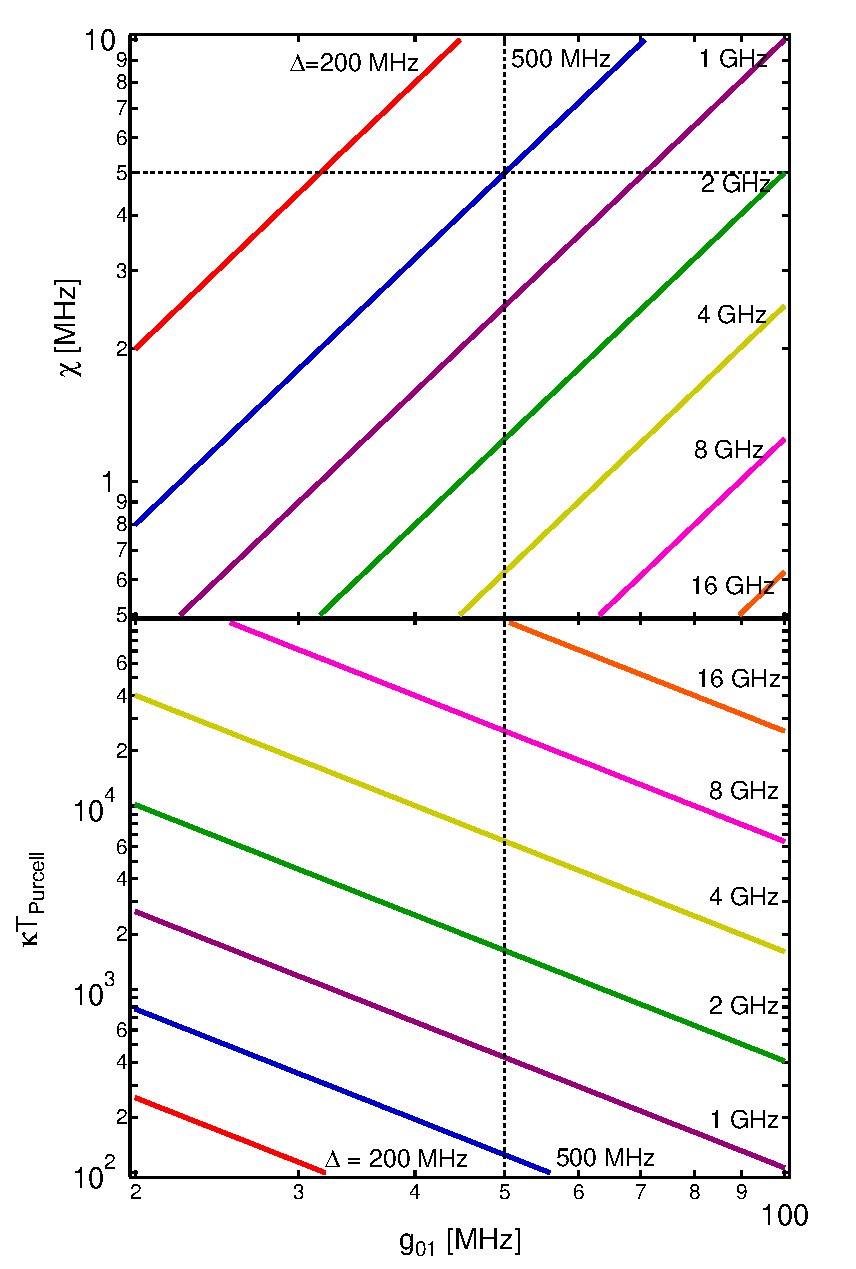
\includegraphics[width=0.6\textwidth]{./material/mathematica/readout_purcell_and_chi_vs_g}
	\caption[]{The dispersive shift $\chi$ of the resonator and the relaxation time $\kappa\cdot T_{Purcell}$ (normalized to the decay rate $\kappa=\omega_r/Q$ of the resonator) of the qubit for a qubit dispersively coupled to a resonator, plotted as a function of the coupling strength $g_{01}$ and shown for different values of the qubit-resonator detuning $\Delta = \omega_{r}-\omega_{01}$.}
	\label{fig:purcell_rate_and_chi}
\end{SCfigure}


To illustrate the effect of $g_{01}$ and $\Delta$ on the relaxation time $T_1$ and the dispersive shift $\chi$, fig. \ref{fig:purcell_rate_and_chi} shows both quantities as a function of $g_{01}$, plotted for several choices of $\Delta$. Now, criterion 1 above demands that the dispersive shift be large enough to completely separate the switching probability distributions for different qubit states. The width of these probability curves can be calculated theoretically, however for this discussion we rely on experimentally measured values and assume that a dispersive shift of $\Delta \chi \approx 5\;\mathrm{MHz}$ suffices to fully separate the two distributions. This assumption limits the range of possible values for $g_{01}$ and $\Delta$ to the region above the horizontal line in fig. \ref{fig:purcell_rate_and_chi}a. On the other hand, criterion 2 demands that the time required to map the qubit state to the oscillator state should be small compared to the relaxation time of the qubit. For the CJBA parameters relevant to this work, this time is given as $T_{meas}\approx 50-100\;\mathrm{ns}$. In order to have negligible qubit relaxation during the readout, we therefore demand that $T_1 \ge 1\;\mathrm{\mu s}$, which corresponds to a 5 \% relaxation probability during the measurement interval. This again limits the choice of possible values of $g_{01}$ and $\Delta$. 

\smallskip

Another important design parameter of the CJBA is the Kerr constant $K$. This constant defines the non-linearity of the resonator and determines the power at which the resonator becomes bistable. Also, the number of photons in the low- and high-amplitude solution of the resonator increases with increasing $K$. Since the dispersive shift of the qubit frequency caused by the resonator is proportional to the number of these photons, choosing a too high $K$ should be avoided since it can induce large displacements of the qubit frequency, thereby recoupling the two qubits of the processor during the readout operation. 

\smallskip

Taking these constraints into account, for the final choice of parameter values we rely on a set of optimized CJBA parameters that have been obtained in an earlier experiment by Mallet {\it et. al.} \citep{mallet_single-shot_2009}. For our processor we choose readout resonator frequencies $\omega_r^1/2\pi = 6.7 \;\mathrm{GHz}$ and $\omega_r^2/2\pi = 6.85\;\mathrm{GHz}$, quality factors $Q^{1,2}=800$, Kerr constants $2\pi K^{1,2}/\omega_r^{1,2}=-2.5\times 10^{-5}$ and qubit-resonator couplings $g_{01}^{1,2}/2\pi=50\;\mathrm{MHz}$. In addition, we choose a detuning $\Delta/2\pi = 500\;\mathrm{MHz}$ for reading out the qubits, yielding a relaxation rate $\Gamma^{Purcell}_1\approx 0.5\;\mathrm{MHZ}$ during readout.

\section{Summary: Qubit and Readout Parameters}

Having discussed the relevant properties of all building blocks of our processor and their dependence on the sample parameters, we choose a full set of these parameters, summarized in table \ref{table:processor_parameters}. The left column contains the processor parameters, the right column the related sample parameters.

\begin{table}
	\centering
	\begin{tabularx}{\textwidth}{r|X|l}
	Parameter & Value & Related Parameters \\ [0.3cm]
	$E_J$ & $h\cdot 28.4\;\mathrm{GHz}$ & $f_{01}=7\;\mathrm{GHz}$, $\alpha=-250\;\mathrm{MHz}$ \\ [0.3cm]
	$E_C$ & $h\cdot 0.92\;\mathrm{GHz}$ & $C_q = 42\;\mathrm{fF}$, $I_c = 57.4 \;\mathrm{nA}$\\ [0.3cm]
	$d$ & $0.35$ & \\ [0.3cm]
	$M_{1,2}$ & $0.25\;\mathrm{pH}$ & \\ [0.3cm]
	$g_{qq}/2\pi$  & $10\;\mathrm{MHz}$ & $C_{qq}=0.45\;\mathrm{fF}$ \\ [0.3cm]
	$g_{01}/2\pi$  & $50\;\mathrm{MHz}$ & $C_{qr}\approx 62.8 \;\mathrm{fF}$ \\ [0.3cm]
	$\omega_r^{1}/2\pi$ & $6.7\;\mathrm{GHz}$ & $L_r^1 = 756\;\mathrm{pH}$, $C_r^1= 497 \;\mathrm{fF}$ \\ [0.3cm]
	$\omega_r^{2}/2\pi$ & $6.85\;\mathrm{GHz}$ & $L_r^2 = 739\;\mathrm{pH}$, $C_r^2= 486 \;\mathrm{pF}$\\ [0.3cm]
	$Q_r^{1,2}$ & $800$ & $C_{in}^{1,2}\approx 17 \;\mathrm{fF}$ \\ [0.3cm]
	$K_r^{1,2}$ & $-2.5\times 10^{-5}$ & $I_{J,r}\approx 2.3 \;\mathrm{\mu A}$ \\ [0.3cm] 
	\end{tabularx}
	\caption[]{The sample parameters chosen for the two-qubit processor. The table contains all independent parameters of the processor as well as the dependent parameters derived from them.}
	\label{table:processor_parameters}
\end{table}

\section{Processor Layout \& Fabrication}

\begin{figure}[ht!]
	\centering
	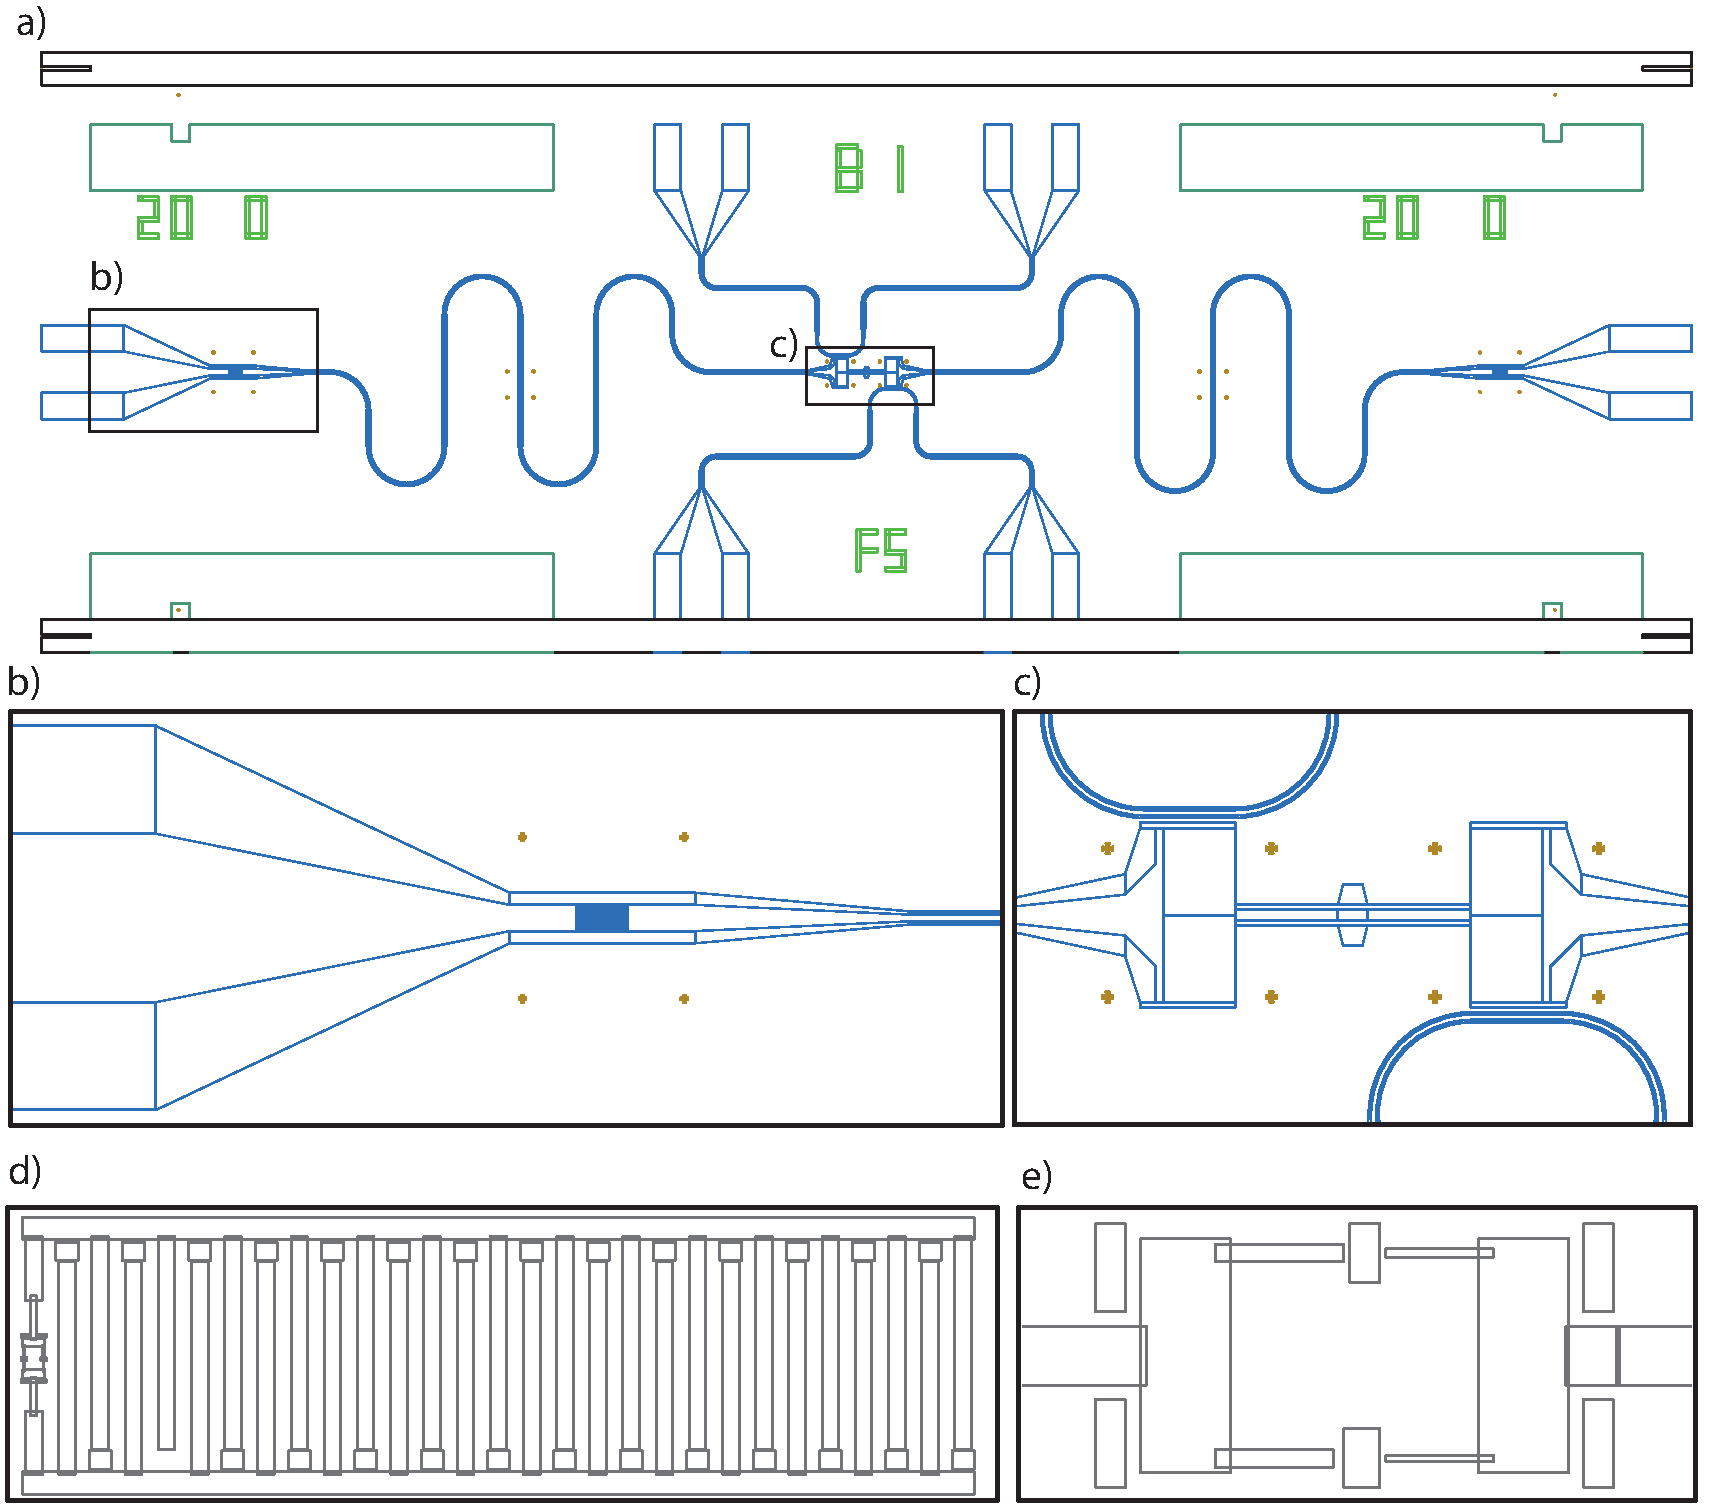
\includegraphics[width=\textwidth]{./material/figures/2-qubit-processor/fabrication/qubit_processor_layout}
	\caption[]{CAD layout schematic of the two-qubit processor, showing the two CPW readout resonators and the two qubits with their adjacent fast flux lines. Subfigures a) and b) show the CAD drawing of the Transmon capacitance and SQUID, as used for the electron beam lithography. Subfigure c) gives a magnified view of the two qubits and their capacitive coupling element, subfigure d) shows the input coupling capacitance of the CPW resonator to the input transmission line.}
	\label{fig:processor_fabrication}
\end{figure}

After having chosen a set of sample parameters, it remains to find a physical implementation of the design that we can realize. In this section we discuss therefore the layout design of the qubit processor. From the beginning, we will restrict our discussion to lithographically fabricated circuits on a chip, disregarding recent approaches to the realization of superconducting qubits and resonators using 3D microwave cavities \citep{paik_observation_2011}.

\smallskip

The readout resonator can be realized as a lumped-elements LC resonator or as a transmission line resonator. In the original approach to CQED \citep{wallraff_strong_2004}, a coplanar waveguide (CPW) resonator was used. Distributed microwave resonators such as CPW resonators are often advantageous since they can be fabricated with a high intrinsic quality factors \citep{megrant_planar_2012,creedon_high_2011,wang_improving_2009,barends_minimal_2010}, although recently large progress has been made concerning the quality factors of discrete LC resonators as well \citep{khalil_loss_2011}. Also, the isolation between the input port of the distributed resonator and the qubit electrode to which the open end of the resonator is coupled is high, whereas for a discrete LC resonator a significant capacitive coupling between the input port of the resonator and the qubit can exist, which is unwanted since it will cause additional relaxation. For this work, we therefore chose a distributed design using a $\lambda/2$ CPW resonator. The open port of the resonator is capacitively coupled to one of the qubit electrodes to achieve the desired coupling factor $g_{01}$.

\smallskip

The flux lines can be realized in several ways. For our processor, we choose a simple 50 $\Omega$ CPW transmission line that is passing nearby the qubit SQUID at a distance of $d\approx 12\;\mathrm{\mu m}$. Since we use the flux line for DC biasing of the qubits as well, shielding currents will flow in the ground planes on either side of the line when a DC current gets applied. These currents can create an unwanted flux bias in the qubit loop and should therefore be eliminated. We achieve this by removing the ground plane between the qubit and the central conductor of the flux line. By doing this, we also increase the capacitive coupling between the line and the qubit electrodes, thereby increasing the charge relaxation rate through the flux line. However, as discussed in section \ref{section:relaxation_through_charge}, for our sample parameters this effect is usually negligible. The flux line can be terminated either directly at the 20 mK stage by wire-bonding it to the ground plane of the chip, or by connecting it to a matched impedance at the 1 K stage of the cryostat. Alternatively, we can also feed back the flux signal to room temperature, which is useful for e.g. measuring the response function of the line.

\smallskip

For the Transmon qubit itself, we need to fabricate a large shunt capacitance $C_J$ in order to achieve the desired charging energy. We implement this capacitance as an interdigitated planar capacitor that we pattern together with the qubit junctions using electron-beam lithography. The Josephson junctions of the qubit are realized in a SQUID geometry with a loop area of $A\approx 16\;\mathrm{\mu m}^2$ and are fabricated using double-angle shadow-evaporation of Aluminium.

\section{Electromagnetic Simulation of the Qubit-Chip}

\begin{figure}[ht!]
	\centering
	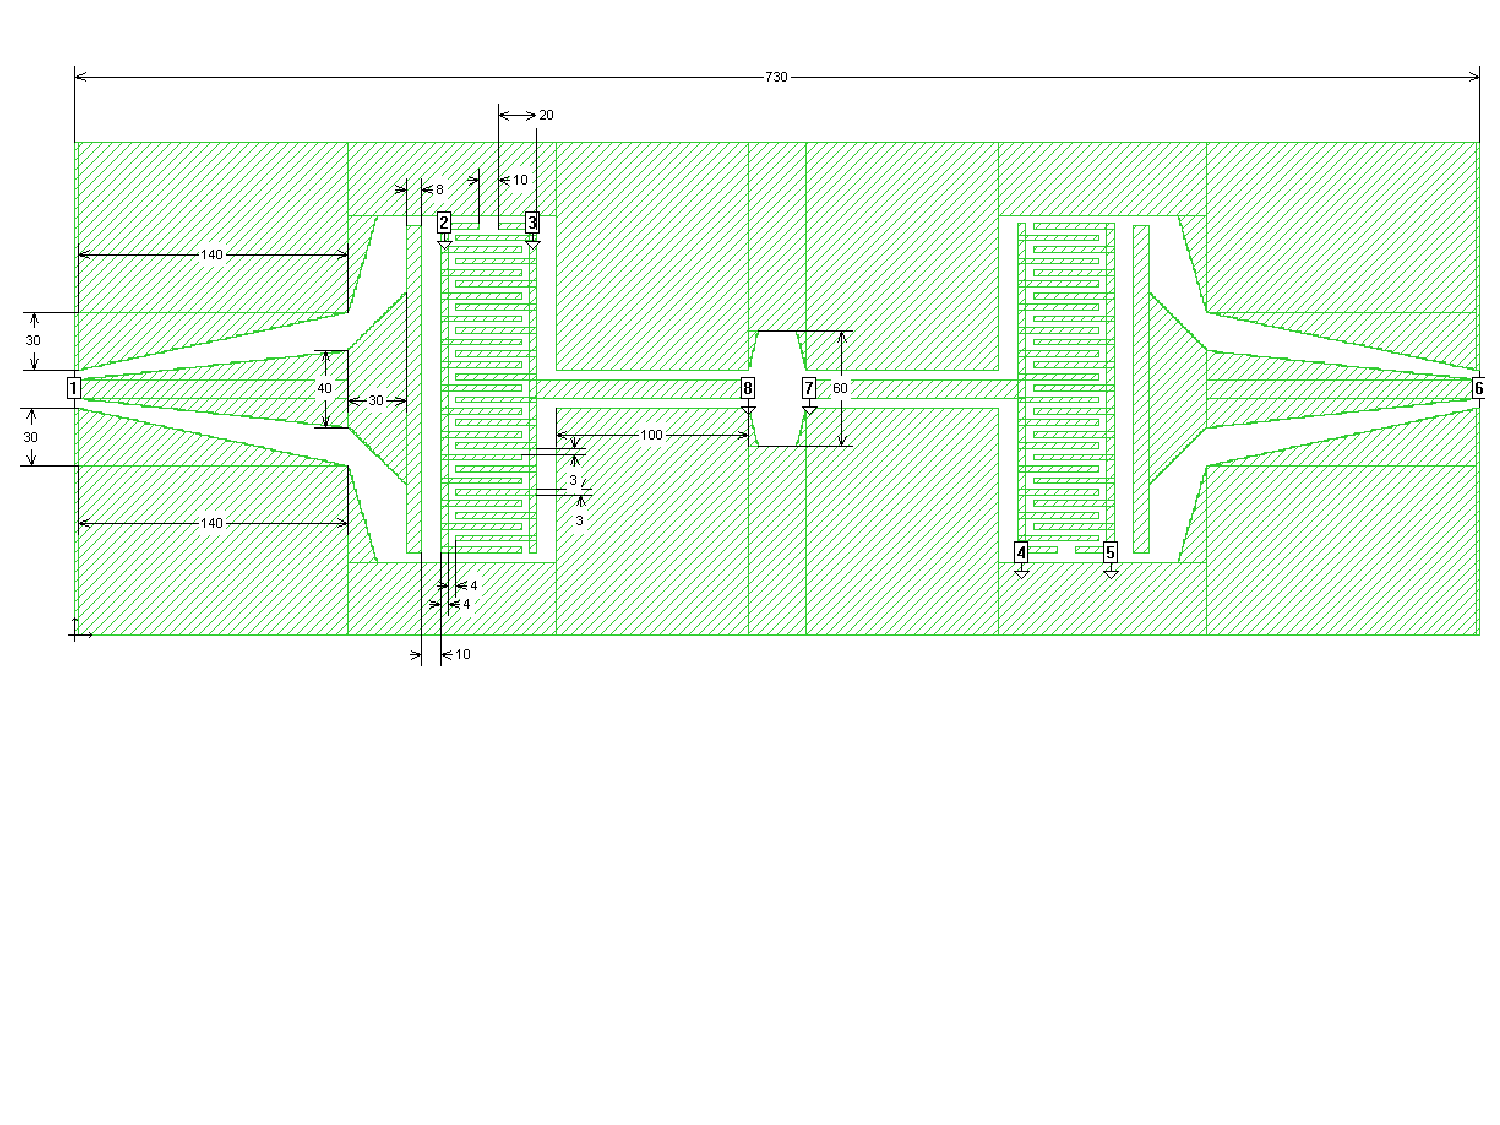
\includegraphics[width=\textwidth]{./material/figures/2-qubit-processor/sonnet_simulation_of_qubit_chip}
	\caption[]{2D model used to model the qubits of the processor using Sonnet microwave simulator (SONNET). Shown are the two Transmon qubit capacitances that are capacitively coupled to each other and to their readout resonator (not shown). Numerical simulation of the circuit yields the capacitances and inductances between all ports of the circuit (1-8).}
	\label{fig:sonnet_model_of_qubit_chip}
\end{figure}

We use a software package for electromagnetic simulation (SONNET) to simulate individual parts of the chip an obtain the transmission coefficients between all relevant circuit components and an equivalent lumped-element model of the circuit. Using this equivalent model we calculate all relevant capacitances and inductances. We can then iteratively adapt the geometry of individual elements in order for them to match the designed parameter values. Fig. \ref{fig:sonnet_generated_model} shows an example of a circuit model generated by this method.

\smallskip

\begin{SCfigure}[1.0][ht!]
	\centering
	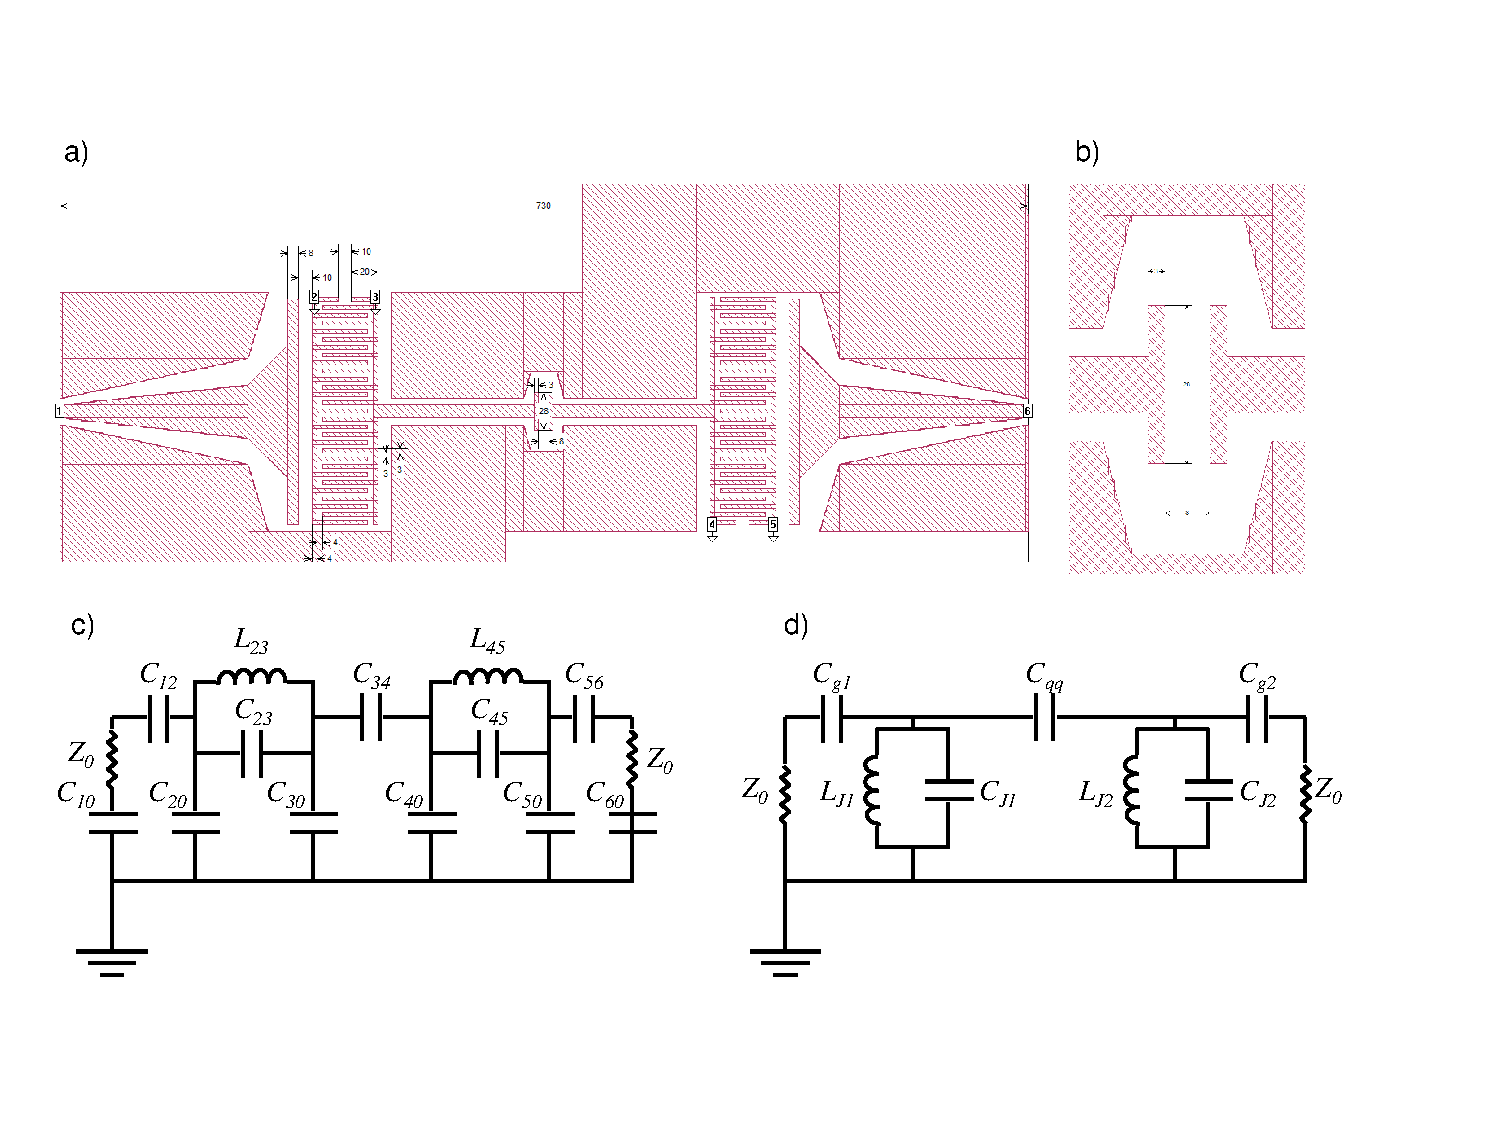
\includegraphics[width=0.6\textwidth]{./material/figures/2-qubit-processor/sonnet_model}
	\caption[]{A circuit model of the geometry shown in fig. \ref{fig:sonnet_model_of_qubit_chip}, generated by SONNET. The parameters of the circuit elements are given as $Z_0=50\;\Omega$, $C_{12}=5.9\;\mathrm{fF}$, $C_{23}=47\;\mathrm{fF}$, $C_{34}=1.2\;\mathrm{fF}$, $C_{45}=47\;\mathrm{fF}$, $C_{56}=5.9\;\mathrm{fF}$, $C_{10}=43\;\mathrm{fF}$, $C_{20}=5\;\mathrm{fF}$, $C_{30}=37\;\mathrm{fF}$, $C_{40}=37\;\mathrm{fF}$, $C_{50}=5\;\mathrm{fF}$, $C_{60}=43\;\mathrm{fF}$, $L_{23}=L_{45}=5.7\;\mathrm{nH}$.}
	\label{fig:sonnet_generated_model}
\end{SCfigure}

We can also simulate the Transmon qubits as harmonic oscillators by modeling their Josephson junction as an inductance that matches the Josephson inductance of the junction, as given by eq. (\ref{eq:josephson_inductance}). By simulating the resonance curve of this harmonic resonator and calculating the corresponding quality factor $Q$, we can estimate the relaxation rate of the qubit through the gate circuit. We can also obtain an estimate of the coupling strength between the two qubits by simulating them as two coupled, linear resonators. We can obtain the impedance seen by the qubit through the gate circuit by this method as well, thereby being able to calculate the corresponding qubit relaxation rate.

\section{Fabrication}

\begin{figure}[p!]
	\includegraphics[width=1\textwidth]{"./material/figures/2-qubit-processor/processor photos"}
	\caption{Optical and electron microscope photos of the two-qubit processor realized in this work (will be replaced with better photos)}
	\label{fig:qubit_chip_photos}
\end{figure}

We fabricate the processor on a high-resistivity silicon substrate with a 50 nm thermal oxide layer. First, we depose 150 nm of Niobium by magnetron sputtering. Afterwards, we spin a photo resist and define an etch mask through optical lithography. Then we dry-etch in a $\mathrm{SF}_6$ plasma, defining the readout resonators, transmission lines and qubit flux lines on the chip. This optical patterning is performed for the wafer as a whole. Afterwards, we spin a bilayer of MAA/PMMA electron beam resist (with typically $1050\;\mathrm{nm}$ of MMA and $115\;\mathrm{nm}$ of PMMA thickness). Then the wafer gets diced and the qubits and JBA junctions are patterned per chip using electron beam lithography, using a double-angle shadow evaporation technique to define the Josephson junctions and capacitances on the chip. The e-beam resist is then lifted off chemically in an Acetone bath. We characterize the chip optically afterwards. In addition, we place ``twin'' structures of the Transmon qubits and the JBAs on each chip that we can use to measure their normal state resistance at room temperature in order to obtain an estimate of the corresponding resistance of the real structures. Giving the normal-state resistance of a Josephson junction we can calculate the Josephson energy by using the Ambegaokar-Baratoff relation
%
\begin{equation}
E_J = \frac{2\pi^2 \Delta}{R_n h},
\end{equation}
%
where $E_J = h I_c / 4\pi e$. When measuring $R_n$ at room temperature, a corrective factor of $\approx 17\%$ has to be applied to the resulting value of $E_J$ to account for variations in $R_n$ with temperature. 

\smallskip

Following we discuss the detailed procedure followed for fabrication of the two-qubit processor chip.

\begin{enumerate}
\item \textbf{Niobium Sputtering}: Deposit 150 nm Niobium at an argon pressure of 1.25 mbar and a power of 0.66 W/cm$^2$ with a 5 minute pre-deposition and $\approx$ 2 min 20 sec deposition time.
\item \textbf{Spinning of Photo-Resist}: Spin S1813 + Shipley Primer at 6000 RPM for 60 sec, bake at 115 ° C for 1 min 15 sec.
\item \textbf{Photo Lithography of Resonators}: Expose the wafer through a contact mask at 5 mW / cm$^2$ for 30 sec.
\item \textbf{Development}: Develop in pure MF 319 for 50 s.
\item \textbf{Reactive Ion Etching}: Pump the RIE chamber to $P\le 4\times 10^{-5}$ mbar. Etch using 20 cc of SF$_6$, 10 cc Ar and 2 cc O$_2$ at a pressure of $\approx$ 0.013 mbar at a power of 50 W and a voltage of 150 V. The total etch time should be $\approx $ 60 sec + 10 sec for the finish. Remove the resists in warm acetone (40 °C) for at least 10 min, possibly clean further in an ultrasonic bath.
\item \textbf{Niobium Surface Regeneration}: Pump the RIE chamber  to $P\le 4\times 10^{-5}$ mbar, etch using 20 cc of SF$_6$, 10 cc Ar at $\approx$ 0.0133 mbar, 50 W and 150 V for 8 sec.
\item \textbf{Electron Resist Spinning}: Spin twice an MAA EL 10 layer at 2000 RPM for 60 sec, 6000 RPM for 2 sec. Bake after each step at 170 °C for 60 sec. Spin PMMA 950k A3 at 4000 RPM for 60 sec, 6000 RPM for 2 sec. Bake at 170 °C for 20 min. This should yield $\approx 1050$ nm of MAA and $110$ nm of PMMA (verify using interferometer).
\item \textbf{Dicing}: Dice the wafer using either a diamond cutter or wafer saw.
\item \textbf{Electron Beam Lithography of Transmons and CJBA junctions}: Clean the chip in iso-propanol (possibly in ultrasound) for less than 2 minutes. Perform electron beam lithography at a dose of $\approx$ 250-320 $\mathrm{\mu C}/cm^2$. Develop the chip in a 1:3 aceton/iso-propanol solution for 50 sec.
\item \textbf{Aluminum Deposition}: Put the sample in the evaporation chamber and pump to $P<10^{-6}$ mbar. Ion mill the sample at the two evaporation angles (typically $\pm 22\deg$) with 500 eV neutralized argon ions at the dose of $2\cdot 10^{15}$/cm$^2$. Deposit first aluminum layer at a rate of 1 nm/sec. Oxidize at an adequate oxygen pressure (typically 15 - 25 mbar) for 10 min. Deposit the second aluminum layer at 1 nm/sec.
\item \textbf{Lift-Off}: Put the chip in a heated Acetone bath at 65 °C for at least 5 min. Rinse in Iso-Propanol. Thermally stabilizee the chip at 100 °C for 1 min.

\end{enumerate}
